\setcounter{chapter}{5} % previous chapter number

\chapter{Stochastic signals and noise}
\label{h:stochastic}

%\setcounter{page}{1}
\minitoc

In this chapter, we will look at optical signals which exhibit a form of randomness. A first type of such stochastic signals are the typical bitstreams that occur in optical communications. Rather than specifying the signal explicitly for all possible bit patterns, it is modelled as a random binary signal where e.g. zeros and ones are equally likely to occur. A second class of randomness encountered in optical signals is the randomness associated with noise, which is obviously unwanted.

Although it is impossible to write down an explicit expression for the waveform of a random signal, such a signal may still exhibit certain regularities when examined over a sufficiently long period of time. These regularities can be described in terms of probabilities, statistical averages, autocorrelation functions, spectral densities ... .

In the first part of this chapter, we will study deterministic signals, before tackling true random signals in the second part. The third and final part deals with a very specific type of random signals, namely noise.
 
\section{Deterministic signals}

\subsection{Energy and power signals}

When transmitting an optical signal, it is converted into an electrical signal at the receiver end. This electrical signal can be represented by either a voltage $v(t)$ or a current $i(t)$, with instantaneous power $p(t)$ across a resistor $R$ given by

\begin{equation}
p(t) = \frac{v^2(t)}{R} = R i^2(t)
\end{equation} 

In communication theory it is often assumed for simplicity that the value of $R$ is unity. With this normalisation convention, we can express the instantaneous power as

\begin{equation}
p(t) =  x^2(t) \label{eq-power}
\end{equation}  

regardless of whether $x(t)$ is a voltage or current signal.

The energy dissipated during a time interval $(-T/2, T/2)$ by a real signal with instantaneous power given by Eq.~\ref{eq-power} can then be written as

\begin{equation}
E_x^T = \int_{-T/2}^{T/2} x^2(t) dt
\end{equation} 

and the \emph{average} power dissipated by the signal during that interval is

\begin{equation}
P_x^T = \frac{1}{T}\int_{-T/2}^{T/2} x^2(t) dt
\end{equation} 

An important class of signals are the so--called \emph{energy signals}. They have a nonzero but finite energy ($0 < E_x < \infty$) for all time, where

\begin{equation}
E_x  = \lim_{T \to \infty}  \int_{-T/2}^{T/2} x^2(t) dt 
\end{equation} 

In the real world, we always transmit signals with finite energy. However, mathematically it is sometimes convenient to consider a different class of signals called \emph{power signals}. These signals have nonzero but finite power ($0 < P_x < \infty$) for all time, where

\begin{equation}
P_x = \lim_{T \to \infty} \frac{1}{T} \int_{-T/2}^{T/2} x^2(t) dt 
\end{equation} 

A typical example of a power signal is a periodic signal stretching from $t=-\infty$ to $t=\infty$. Another example is the mathematical abstraction of a noise signal, which is also assumed to run from $t=-\infty$ to $t=\infty$.

\begin{sidebar}
\begin{ex}
Show that the definitions of power and energy signals are mutually exclusive, i.e. an energy signal can never be a power signal and vice versa.
\end{ex}
\end{sidebar}

\subsection{Spectral density}

It is often interesting to study the properties of a signal in the frequency domain. This concept is particularly important when looking at filters in a telecommunication system. For these purposes, we want to known the spectral content of the signal.

The fourier transform $X(f)$ of the signal $x(t)$ is given by \footnote{In this chapter we will work with the fourier transform with respect to $f$, instead of with the transform with respect to $\omega$ we used earlier. This also has the advantage that the expressions for forward and inverse transform are more symmetrical.}

\begin{equation}
X(f) = \int_{-\infty}^{\infty} x(t) e^{-j 2 \pi f t} dt \label{eq-fourier}
\end{equation} 

Let's suppose for the moment that $x(t)$ is an energy signal. We know from Parceval's theorem that we can write

\begin{equation}
E_x = \int_{-\infty}^{\infty} x^2(t) dt = \int_{-\infty}^{\infty}  \left | X(f) \right |^2 df
\end{equation} 

In other words, the energy of a signal can be calculated both in the frequency and the time domain. 

Let us define $\Psi_x$ as

\begin{equation}
\fbox{$\displaystyle
\Psi_x(f) \stackrel{def}{=} \left | X(f) \right |^2
$}
\end{equation} 

This quantity is called the \emph{energy spectral density} (ESD) of the signal $x(t)$.

For power signals, we need to adapt the definition slightly. Let's call $x_T(t)$ the truncated version of the signal $x(t)$ by observing it only in the interval ($-T/2,T/2$) and setting it to zero everywhere else. The \emph{power spectral density} (PSD) is then defined as

\begin{equation}
G_x(f) \stackrel{def}{=}  \lim_{T \to \infty }\frac{1}{T}\left | X_T(f) \right |^2 \label{eq-psd}
\end{equation} 

For the special case where $x(t)$ is a periodic function with frequency $f$, the PSD consists of a set of delta peaks at $n f$.

The quantity $\left | X_T(f) \right |^2 / T$ is often called a \emph{periodogram} of the signal.

\subsection{Autocorrelation function}

Autocorrelation refers to matching a signal with a delayed version of itself. The autocorrelation function $R_x(\tau)$ of a real--valued energy signal $x(t)$ is defined as

\begin{equation}
\fbox{$\displaystyle
R_x(\tau) = \int_{-\infty}^{\infty}x(t)x(t+\tau)dt \label{autocor}
$}
\end{equation} 

This function provides a measure of how closely the signal matches a copy of itself as the copy is shifted $\tau$ units in time. $R_x(\tau)$ is not a function of time, only of the time difference $\tau$ between the waveform and its shifted copy.

The autocorrelation function has some properties which are easily proven:

\begin{enumerate}
\item
$R_x(\tau) = R_x(-\tau)$
\item
$R_x(0) = E_x$
\end{enumerate}

For a power signal, the autocorrelation function is defined as

\begin{equation}
R_x(\tau) = \lim_{T \to \infty} \frac{1}{T} \int_{-T/2}^{T/2} x(t)x(t+\tau)dt
\end{equation} 

\subsection{Wiener--Khinchin theorem}

The Wiener--Khinchin theorem relates the autocorrelation function to the energy spectral density of an energy signal.

By taking the inverse of Eq.~\ref{eq-fourier}, we can write

\begin{equation}
x(t) = \int_{-\infty}^{\infty} X(f) e^{j 2 \pi f t} df
\end{equation}

Plugging this in the definition of the autocorrelation function Eq.~\ref{autocor}, we get 

\begin{equation}
R_x(\tau) = \int_{-\infty}^{\infty} \left[ \int_{-\infty}^{\infty} X(f) e^{j 2 \pi f t} df \right] \left[ \int_{-\infty}^{\infty} X(f') e^{j 2 \pi f' (t+\tau)} df' \right]dt
\end{equation} 

This can be rearranged as

\begin{equation}
R_x(\tau) = \int_{-\infty}^{\infty}  \int_{-\infty}^{\infty} \int_{-\infty}^{\infty} X(f)X(f') e^{j 2 \pi (f+f') t}   e^{j 2 \pi f' \tau} df df' dt
\end{equation} 

Evaluating the integral with respect to $t$, we get

\begin{equation}
R_x(\tau) = \int_{-\infty}^{\infty}  \int_{-\infty}^{\infty}  X(f)X(f') \delta(f+f')   e^{j 2 \pi f' \tau} df df'
\end{equation} 

So, $f'=-f$ or

\begin{equation}
R_x(\tau) = \int_{-\infty}^{\infty} X(f)X(-f) e^{-j 2 \pi f \tau} df 
\end{equation} 

For real signals $x(t)$, it is easy to prove that $X(-f)=X^*(f)$, so

\begin{equation}
\fbox{$\displaystyle
R_x(\tau) = \int_{-\infty}^{\infty} |X(f)|^2 e^{-j 2 \pi f \tau} df \label{eq-wiener}
$}
\end{equation} 

In other words, the autocorrelation function and the energy spectral density form a fourier transform pair!

It can also be understood intuitively that the autocorrelation function contains information about the spectral content of the signal. If the autocorrelation function changes slowly when $\tau$ is increased from zero, it means that sample values at $t=t_1$ and $t=t_1+\tau$ will be roughly the same. Thus, we'd expect the frequency domain representation of the signal to contain predominantly low frequencies.

If on the other hand the autocorrelation function drops sharply when $\tau$ is increased, we would expect the signal to change rapidly over time and therefore to have a high--frequency spectral content.

\section{Stochastic signals}

All useful message signals appear random: the receiver does not know beforehand which of the possible waveforms will be transmitted. Therefore, we need to be able to form efficient descriptions of random signals.

\subsection{Random variables}

Consider a random variable $X$ at a fixed moment in time. This variable is described by its \emph{probability density function} (pdf) $p_X(x)$ as follows:

\begin{equation}
P(x_1 \le X \le x_2) = \int_{x_1}^{x_2}p_X(x) dx
\end{equation} 

$p_X(x)$ is a non--negative function, and the total area under its curve is equal to unity.

The \emph{mean value} or \emph{expected value} of a random variable $X$ is defined by

\begin{equation}
m_X = {\bf E}\{ X \} = \int_{-\infty}^{\infty}x p_X(x) dx
\end{equation} 

Here, ${\bf E}\{ . \}$ is called the \emph{expected value operator}.

If we don't know the probability density function, the only (hypothetical) way to estimate the expected value would be to replicate our system many times over, so that we have an enormous number of systems which are all governed by the same statistics. Such a (hypothetical) collection of replicated systems is called an \emph{ensemble}. By observing each of the replicas and averaging the results, we can get an idea of the expected value. This process is called \emph{ensemble averaging}.

\subsection{Random processes}

If we have a random variable $X$ that evolves over time, we get a a \emph{random process} or a \emph{random signal} $X(t)$. In its most general form, its probability density function will be different for different moments in time: $ p_X(x) = p_{X,t}(x)$.

The mean of a random process is defined by

\begin{equation}
m_X(t) = {\bf E}\{ X(t) \} = \int_{-\infty}^{\infty}x p_{X,t}(x) dx
\end{equation} 

and is in general a function of time.

The autocorrelation of a random signal is defined by

\begin{equation}
R_X(t,\tau) = {\bf E}\{ X(t)X(t+\tau) \}
\end{equation} 

\subsection{Stationarity}

A random signal $X(t)$ is said to be \emph{stationary} if none of its statistics change over time.

If only the mean and the autocorrelation of a signal are time--invariant, we call the process \emph{wide--sense stationary}, which is a much relaxed requirement.

In telecommunication, we often assume that our signal are wide--sense stationary. In this case, we have

\begin{equation}
m_X(t) = m_X
\end{equation} 

and

\begin{equation}
R_X(t,\tau) = R_X(\tau) = {\bf E}\{ X(t) X(t+\tau) \}
\end{equation} 

If instead of a continuous signal $X(t)$, we are dealing with a discrete set of events $\{ a_n \}$, also wide--sense stationary, the autocorrelation becomes

\begin{equation}
R_a(m) = {\bf E}\{ a_n a_{n+m} \}
\end{equation} 

\subsection{Ergodicity}

A more stringent requirement than stationarity is that of ergodicity. When a random process is \emph{ergodic}, its time averages equal its ensemble averages. So, in order to estimate e.g.
the expected value, instead of constructing an ensemble of replicated systems and observing those, we can study a single sample system and calculate a time average of its behaviour.

An ergodic system is always stationary in the strict sense, although the opposite is not necessarily true.

Rather than having ergodicity for all of its statistical parameters, we can also have systems which are only ergodic with respect to the mean and/or the correlation function.

A system is \emph{ergodic in the mean} if

\begin{equation}
m_X = \lim_{T \to \infty} \frac{1}{T} \int_{-T/2}^{T/2} X(t) dt
\end{equation} 

A system is \emph{ergodic in the autocorrelation function} if

\begin{equation}
R_X(\tau) = \lim_{T \to \infty} \frac{1}{T} \int_{-T/2}^{T/2} X(t) X(t+\tau) dt
\end{equation} 

Testing for ergodicity of a random signal is usually very difficult. In practice one makes an intuitive judgement as to whether it is reasonable to interchange the time and ensemble averages.

\subsection{Power spectral density}

Consider a random signal $X(t)$ with power spectral density $G_X(f)$. Although we don't prove it here explicitly, we can start from the definition of power spectral density Eq.~\ref{eq-psd} and write down something similar to the Wiener--Khinchin theorem Eq.~\ref{eq-wiener}:

\begin{equation}
G_X(f) = \int_{-\infty}^{\infty} R_X(\tau) e^{j 2 \pi f \tau} d \tau \label{eq-wiener-random}
\end{equation} 

\begin{figure}
\centering
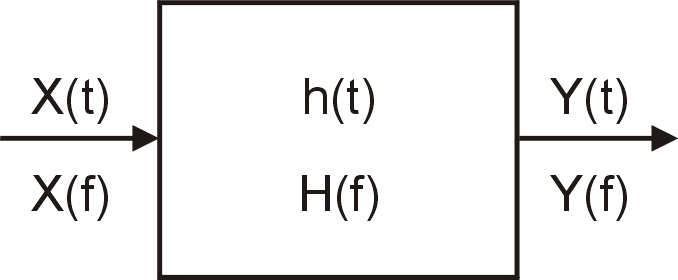
\includegraphics{stochastic/figures/linsys}
\caption{A linear system.}
\label{fig-linsys}
\end{figure}

Let's now investigate what happens if we use $X(t)$ as input to a linear system (see Fig.~\ref{fig-linsys} ). We know from systems theory that if a linear system has impulse response $h(t)$, the output $Y(t)$ is given by the following convolution:

\begin{equation}
Y(t) = h(t) \otimes X(t) = \int X(\tau) h(t-\tau) d \tau
\end{equation} 

In the frequency domain, this becomes

\begin{equation}
Y(f) = H(f) X(f)
\end{equation} 

with $H(f)$ the frequency response of the system. So, for the power spectral density at the output we get (once again without formal proof, but the result should be intuitively acceptable from Eq.~\ref{eq-psd}) :

\begin{equation}
G_Y(f) = \left | H(f) \right | ^ 2 G_X(f)
\end{equation}
 
\subsection{Baseband digital signals}

\subsubsection{Power spectral density}

A baseband digital signal can be expressed as

\begin{equation}
X(t) = \sum_{n=-\infty}^{\infty}a_n h(t-nT)
\end{equation} 

Here, $\{ a_n \}$ is discrete random sequence of signal levels, which could be binary or multilevel. $h(t)$ is the pulse waveform used (e.g. a rectangular pulse) and $T$ is the period.

To calculate the power spectral density of such a signal, we start by observing that this signal can be obtained by taking a train of dirac pulses

\begin{equation}
X_0(t) = \sum_{n=-\infty}^{\infty}a_n \delta(t-nT)
\end{equation} 

and sending it through a system with impulse response $h(t)$. Therefore, the power spectral density of $X(t)$ can be written as

\begin{equation}
G_X(f) = \left | H(f) \right |^2 G_{X_0}(f)
\end{equation} 

We still have to determine $G_{X_0}(f)$. To do this, we will first calculate the autocorrelation function and then take a fourier transform. For the autocorrelation function we get

\begin{equation}
R_{X_0}(\tau) = {\bf E}\{X_0(t) X_0(t+\tau)\}
\end{equation}

If $\tau$ is not a multiple of $T$, the two pulse trains will never overlap and the autocorrelation will be zero. This means that $R_{X_0}(\tau)$ is only non--zero when $\tau=nT$:

\begin{equation}
R_{X_0}(\tau) = \sum_{k=-\infty}^{\infty}R_k \delta(\tau-kT)
\end{equation} 

Here, the coefficients $R_k$ are actually none other than the autocorrelation functions for the discrete random series $\{ a_n \}$:

\begin{equation}
R_{X_0}(\tau) = \sum_{k=-\infty}^{\infty} {\bf E} \{ a_n a_{n+k} \} \delta(\tau-kT)
\end{equation} 

So, by using Eq.~\ref{eq-wiener-random}:

\begin{equation}
G_{X_0}(f) = \int_{-\infty}^{\infty} \left ( \sum_{k=-\infty}^{\infty} {\bf E} \{ a_n a_{n+k} \} \delta(\tau-kT) \right ) e^{j 2 \pi f \tau} d \tau 
\end{equation} 

This simplifies to

\begin{equation}
G_{X_0}(f) =  \sum_{k=-\infty}^{\infty} {\bf E} \{ a_n a_{n+k} \}   e^{j 2 \pi f k T} 
\end{equation} 

So, finally

\begin{equation}
\fbox{$\displaystyle
G_X(f) =  \left | H(f) \right |^2 \sum_{k=-\infty}^{\infty} {\bf E} \{ a_n a_{n+k} \}   e^{j 2 \pi f k T} \label{eq-bb-psd}
$}
\end{equation} 

\subsubsection{Non--return--to--zero modulation}

As an example, let's look at non--return--to--zero (NRZ) modulation, where 'one' is represented by a rectangular pulse of duration $T$ and amplitude $A$. 'Zero' is represented by the absence of a pulse (Fig.~\ref{fig-nrz}).

\begin{figure}
\centering
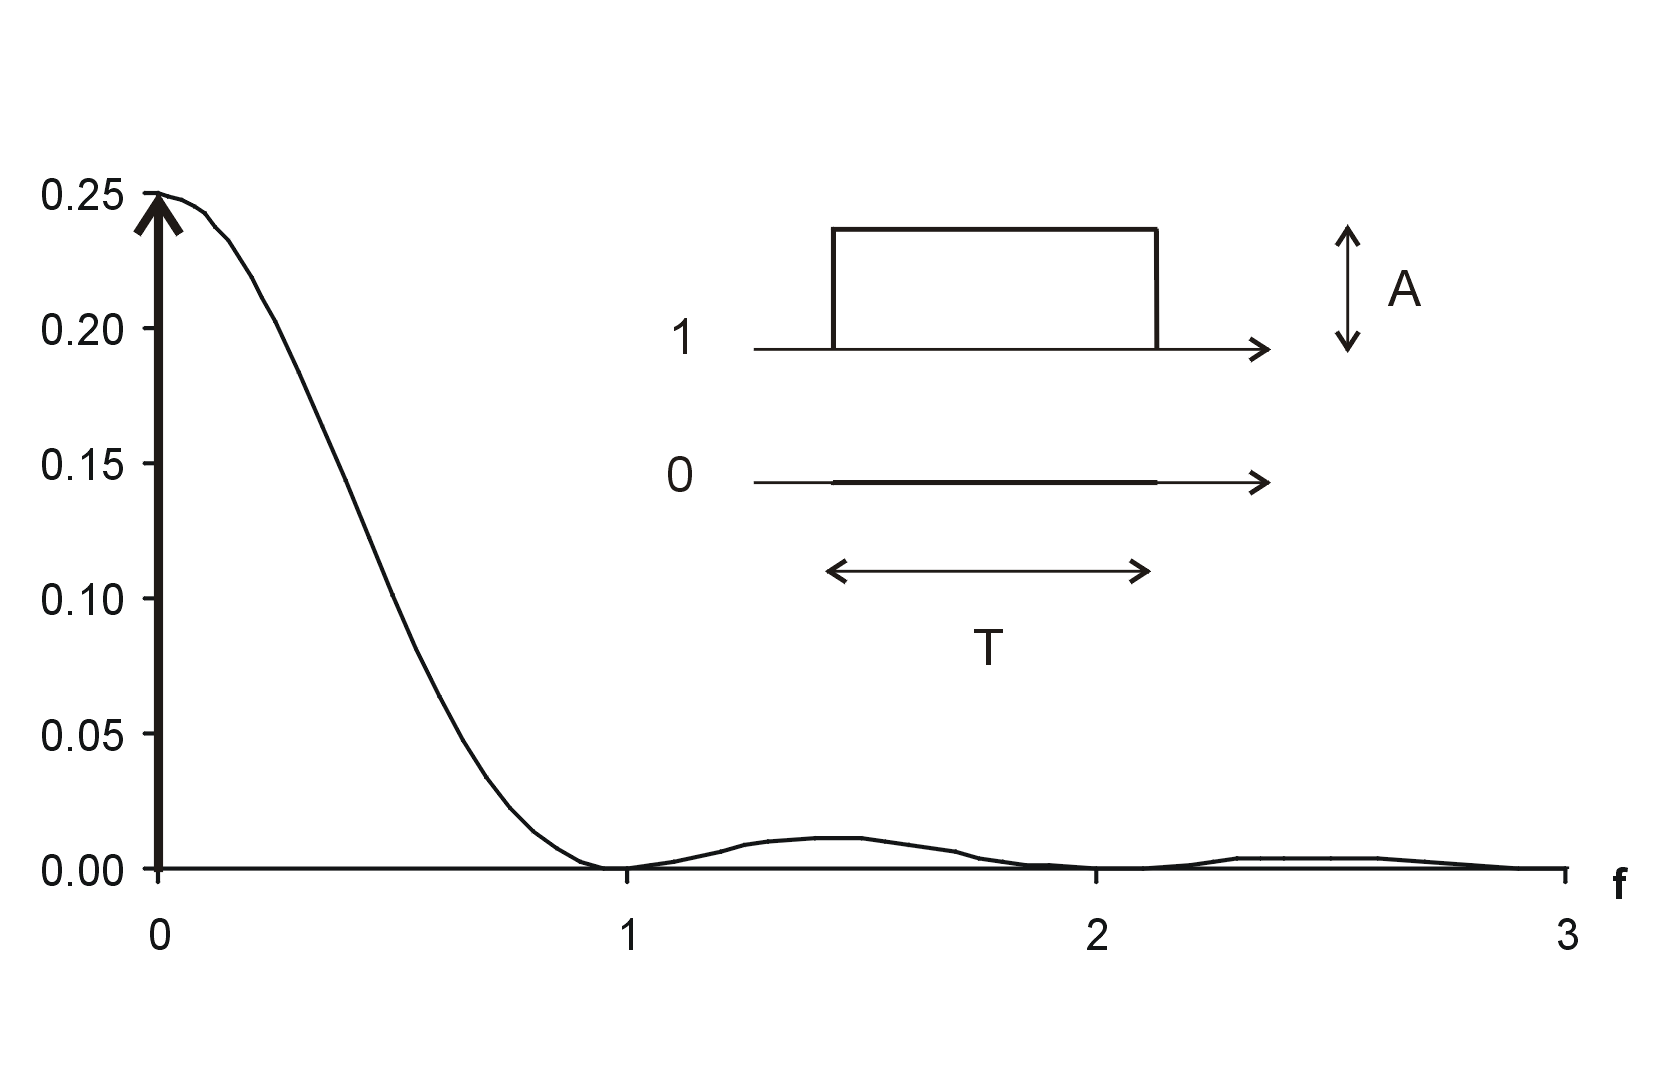
\includegraphics[width=10cm]{stochastic/figures/nrz}
\caption{The non--return--to--zero modulation format. The power spectral density is plotted for $A=T=1$.}
\label{fig-nrz}
\end{figure}

Such a rectangular pulse is described by

\begin{equation}
h(t) = 
\begin{cases}
1, \hspace{0.5cm} {\rm for } \hspace{0.1cm} 0 < x < T \\ 
0, \hspace{0.5cm} {\rm otherwise}
\end{cases}
\end{equation} 

for which

\begin{equation}
\left | H(f) \right |^2 = T^2 {\rm sinc}^2 (f T)
\end{equation} 

where ${\rm sinc} (x) = \sin (\pi x) / \pi x$.

$\{ a_n \}$ is a random sequence of values from $\{A, 0\}$ both with equal probability. So, for the autocorrelation we get

\begin{align}
R_a(0) &= {\bf E}(a_n a_n) \\ \nonumber
       &= (0)(0) P(a_n=0, a_n=0) \\ \nonumber
       &+ (A)(A)P(a_n=A, a_n=A) \\ \nonumber 
       &= \frac{A^2}{2}
\end{align} 

Similarly,

\begin{align}
R_a(m) &= {\bf E}(a_n a_{n+m}) \\ \nonumber
       &=  (0)(0) P(a_n=0, a_{n+m}=0) \\ \nonumber
         & + (0)(A) P(a_n=0, a_{n+m}=A) \\ \nonumber
	 & + (A)(0)P(a_n=A, a_{n+m}=0) \\ \nonumber      
	 & + (A)(A)P(a_n=A, a_{n+m}=A) \\ \nonumber
	&= \frac{A^2}{4}
\end{align}

Plugging all of this in Eq.~\ref{eq-bb-psd} and rewriting $R_a(0) = A^2/4 + A^2/4$, we get

\begin{equation}
G_X(f) =  T^2 {\rm sinc}^2 (f T) \left [ \frac{A^2}{4} + \sum_{k=-\infty}^{\infty} \frac{A^2}{4}  e^{j 2 \pi f k T} \right ]
\end{equation} 

\begin{sidebar}
\begin{ex}
Show that 
$$\sum_{k=-\infty}^{\infty}  e^{j 2 \pi f k T} = \frac{1}{T} \sum_{k=-\infty}^{\infty} \delta(f-\frac{k}{T})$$

Hint: the right--hand side is a periodic function in $f$ with period $1/T$. Write it as a fourier series of complex exponentials.
\end{ex}
\end{sidebar}

Using this result, we get

\begin{equation}
G_X(f) =  \frac{A^2 T^2}{4} {\rm sinc}^2 (f T) \left [ 1 + \frac{1}{T} \sum_{k=-\infty}^{\infty} \delta(f-\frac{k}{T}) \right ] \label{eq-nrz}
\end{equation} 

Multiplying a function $f(x)$  with $\delta(x-x_0)$ is equivalent to $f(x_0)\delta(x-x_0)$, so

\begin{equation}
G_X(f) =  \frac{A^2 T^2}{4} {\rm sinc}^2 (f T)  + \frac{A^2T}{4} \sum_{k=-\infty}^{\infty} {\rm sinc}^2 (k)  \delta(f-\frac{k}{T}) 
\end{equation} 

Since ${\rm sinc}^2 (k)$ is zero for $k \ne 0$, and one for $k=0$, we finally get

\begin{equation}
\fbox{$\displaystyle
G_X(f) =  \frac{A^2 T^2}{4} {\rm sinc}^2 (f T)  + \frac{A^2T}{4} \delta(f)
$}
\end{equation} 

The result is also plotted in Fig.~\ref{fig-nrz}. Note the dc spike.

\subsection{Return--to--zero modulation}

This modulation format is plotted in Fig.~\ref{fig-rz}. It is identical to NRZ, except for the fact that the waveform is now given by

\begin{figure}
\centering
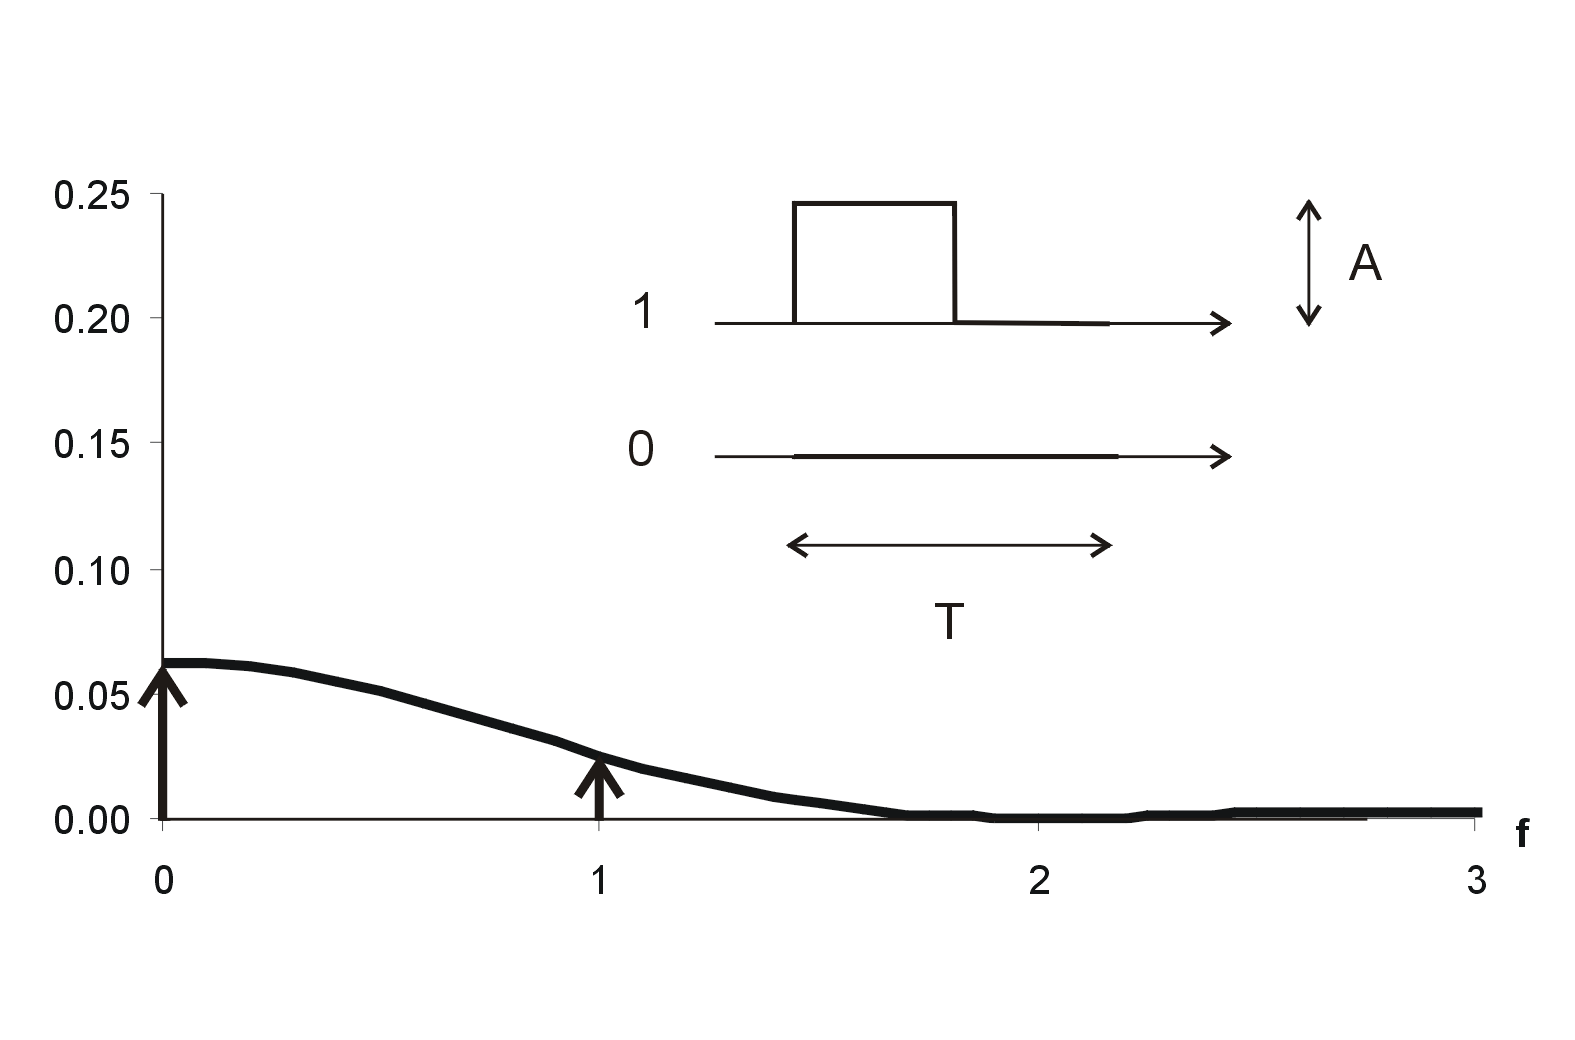
\includegraphics[width=10cm]{stochastic/figures/rz}
\caption{The return--to--zero modulation format. The power spectral density is plotted for $A=T=1$.}
\label{fig-rz}
\end{figure}


\begin{equation}
h(t) = 
\begin{cases}
1, \hspace{0.5cm} {\rm for } \hspace{0.1cm} 0 < x < T/2 \\ 
0, \hspace{0.5cm} {\rm otherwise}
\end{cases}
\end{equation} 

for which

\begin{equation}
\left | H(f) \right |^2 = \frac{T^2}{4} {\rm sinc}^2 (f \frac{T}{2})
\end{equation} 

Making the necessary modifications to Eq.~\ref{eq-nrz}, we get

\begin{equation}
G_X(f) =  \frac{A^2 T^2}{16} {\rm sinc}^2 (\frac{f T}{2}) \left [ 1 + \frac{1}{T} \sum_{k=-\infty}^{\infty} \delta(f-\frac{k}{T}) \right ]
\end{equation} 

This becomes

\begin{equation}
G_X(f) =  \frac{A^2 T^2}{16} {\rm sinc}^2 (\frac{f T}{2}) +  \frac{A^2 T}{16} \sum_{k=-\infty}^{\infty}{\rm sinc}^2 (\frac{k}{2}) \delta(f-\frac{k}{T})
\end{equation} 

The result is also plotted in Fig.~\ref{fig-rz}. Note the discrete spikes for $k=0$ and for odd values of $k$.

\section{Noise}

\subsection{Classification of noise}

Noise is the general term given to unwanted fluctuations in the received signal which do not carry any information. Noise can be caused by a variety of reasons: thermal effects, effects related to the discrete character of electrons and photons, ... .

In general, noise can be classified according to several (independent) criteria.

The first one is whether or not the noise statistics are \emph{stationary}, i.e. invariant in time. When modelling noise, it is mostly assumed that noise is stationary.

A second criterion is related to the nature of the \emph{power density spectrum}, which as we know is the fourier transform of the autocorrelation function. For noise that is totally uncorrelated, i.e. the noise at $t=t_0+\epsilon$ is completely uncorrelated to the noise at $t=t_0$, the autocorrelation function will be a delta spike at $\tau=0$. The fourier transform of this is a constant function, i.e. the noise contains an equal fraction of frequencies from dc up to infinity. This is obviously not possible in reality, but this so--called \emph{white noise} is still a useful mathematical abstraction to model noise.

A third criterion relates to the \emph{probability density function} that generates the noise at each time instant $t$. E.g. for a gaussian pdf we talk about gaussian noise, for a poisson pdf we talk about poisson noise. Note that this is completely unrelated to the previous criterion, which dealt with the correlation between different time instants, whereas this criterion deals with noise statistics at an isolated time instant.

We will now discuss some of the most common types of noise in photonic systems.

\subsection{Thermal noise}

Thermal noise is actually the most common type of noise, and is generated by the thermal agitation of carriers in light sources and detectors. It is usually modelled as a term $n$ with zero average which is added to the signal. This noise has a gaussian pdf:

\begin{equation}
p(n) = \frac{1}{\sigma \sqrt{2 \pi}} e^{-\frac{n^2}{2 \sigma^2}}
\end{equation} 

Here, $\sigma^2$ is the variance of $n$.

It is also assumed that this noise is completely uncorrelated and hence white.

Summarising all this features leads to the term \emph{additive white gaussian noise} (AWGN).

\subsection{Shot noise}

Shot noise is a different kind of noise, which is related to the quantum nature of light. At low light intensities, the light beam can be modelled as a discrete process in which a sequence of photons arrives at the detector. The interval between different arrivals is obviously subjected to some kind of randomness, which gives rise to noise.

The statistics are governed by a poisson process with pdf

\begin{equation}
p(n) = \frac{\mu^{-n}e^{-\mu}}{n!}
\end{equation}  

Here, $\mu$ is the mean value as well as the variance.

Another consequence of this type of noise stems from one of the uncertainty relations of Heisenberg, which links an uncertainty on the number of photons to an uncertainty on their phase. Thus, the discrete character of photons also inevitably gives rise to \emph{phase noise}, i.e. uncertainty on the phase of the light beam.

\pagebreak
\section*{Norbert Wiener (1894--1964)}

\parpic{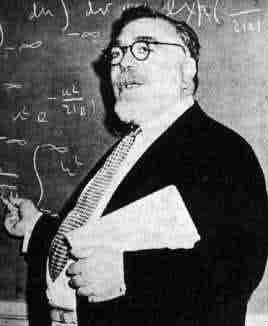
\includegraphics[width=7cm]{stochastic/figures/wiener}}

Norbert Wiener bas born 26 Nov 1894 in Columbia, Missouri, USA. He writes in about his upbringing as follows: "I was brought up in a house of learning. My father was the author of several books, and ever since I can remember, the sound of the typewriter and the smell of the paste pot have been familiar to me. ... I had full liberty to roam in what was the very catholic and miscellaneous library of my father. At one period or other the scientific interests of my father had covered most of the imaginable subjects of study. ... I was an omnivorous reader ..."

Wiener had problems regarding his schooling, partly because the reading which he had done at home had meant that he was advanced in certain areas but much less so in others. His parents sent him to the Peabody School when he was seven years old and, after worrying about which class he should enter, had him begin in the third grade. After a short time his parents and teachers felt he would be better suited to the fourth grade and he was moved up a year. However, he certainly did not fit into the school in either grade and his teacher had little sympathy with so young a boy in the fourth grade yet lacking certain skills which would be expected the pupils at this stage in their education. 

From this time on Wiener's father took over his education and he made rapid progress for so young a child. However, Wiener had problems relating to his movements and was obviously very clumsy. This stemmed partly from poor coordination but also partly for poor eyesight. Advised by a doctor to stop reading for six months to allow his eyes to recover, he still had regular lessons from his father who now taught him to do mathematics in his head. After the six months were up Wiener went back to reading but he had developed some fine mental skills during this period which he retained all his life. 

In September 1906, still only eleven years old, Wiener entered Tufts College. Socially a child, he was an adult in educational terms so his student days were not easy ones. Although taking various science courses, he took a degree in mathematics.  Having won a scholarship to Cornell he entered in 1910 at the age of 15 to begin graduate studies in philosophy. Taking mathematics and philosophy courses, Wiener did not have a successful year and before it was finished his father had made the necessary arrangements to return to Harvard to continue philosophy. 

Back at Harvard Wiener was strongly influenced by the fine teaching of Edward Huntington on mathematical philosophy. He received his Ph.D. from Harvard at the age of 18 with a dissertation on mathematical logic supervised by Karl Schmidt. He taught philosophy courses at Harvard in 1915, worked for a while for the General Electric Company, then joined Encyclopedia Americana as a staff writer in Albany. While working there he received an invitation from Veblen to undertake war work on ballistics at the Aberdeen Proving Ground in Maryland. Taking about mathematics with his fellow workers while undertaking this war work revived his interest in mathematics. At the end of the war Osgood told him of a vacancy at MIT and he was appointed as an instructor in mathematics. 

His first mathematical work at MIT led him to examine Brownian motion. In fact, as Wiener explained, this first work would provide a connecting thread through much of his later studies: "... this study introduced me to the theory of probability. Moreover, it led me very directly to the periodogram, and to the study of forms of harmonic analysis more general than the classical Fourier series and Fourier integral. All these concepts have combined with the engineering preoccupations of a professor of the Mathematical Institute of Technology to lead me to make both theoretical and practical advances in the theory of communication, and ultimately to found the discipline of cybernetics, which is in essence a statistical approach to the theory of communication. Thus, varied as my scientific interests seem to be, there has been a single thread connecting all of them from my first mature work ... "

Wiener's papers were hard to read. Sometimes difficult results appeared with hardly a proof as if they were obvious to Wiener, while at other times he would give a lengthy proof of a triviality. Despite the style of his papers, Wiener contributed some ideas of great importance. We have already mentioned above his work in 1921 in Brownian motion. He introduced a measure in the space of one dimensional paths which brings in probability concepts in a natural way. From 1923 he investigated Dirichlet's problem, producing work which had a major influence on potential theory. 

Wiener's mathematical ideas were very much driven by questions that were put to him by his engineering colleagues at MIT. These questions pushed him to generalise his work on Browian motion to more general stochastic processes. This in turn led him to study harmonic analysis in 1930. His work on generalised harmonic analysis led him to study Tauberian theorems in 1932 and his contributions on this topic won him the Bocher Prize in 1933.

Wiener had an extraordinarily wide range of interests and contributed to many areas in addition to those we have mentioned above including communication theory, cybernetics (a term he coined), quantum theory and during World War II he worked on gunfire control. It is probably this latter work which motivated his invention of the new area of cybernetics which he described in Cybernetics: or, Control and Communication in the Animal and the Machine (1948). 

Freudenthal describes both Wiener's appearance and his character: "In appearance and behaviour, Norbert Wiener was a baroque figure, short, rotund, and myopic, combining these and many qualities in extreme degree. His conversation was a curious mixture of pomposity and wantonness. He was a poor listener. His self--praise was playful, convincing and never offensive. He spoke many languages but was not easy to understand in any of them. He was a famously bad lecturer." 

(Based on J. O'Connor and E. Robertson from http://www--gap.dcs.st--and.ac.uk/)